\chapter{Suffixbomen}\label{ch:suffix-bomen}
Een eerste datastructuur die het mogelijk maakt om snel kleine strings in een groot aantal andere strings op te zoeken zijn suffixbomen.
Meer precies eigenlijk een gegeneraliseerde suffixboom.
\\ \\
We behandelen deze datastructuur als eerste omdat hij vrij intuïtief is en de makkelijkste van alle mogelijke opties.
Bovendien kan een goede tijdscomplexiteit bereikt worden aangezien het zoeken in een suffixboom in $O(n)$ tijd kan (met $n$ de lengte van de zoekstring, in ons geval is dit een peptide).
Het opbouwen van de suffixboom kan ook in lineaire tijd gebeuren, al zei het dan lineair in de totale lengte van alle proteïnen in de databank (die we aanduiden met $m$).

\section{Wat zijn suffixbomen?}\label{sec:wat-zijn-suffix-bomen?}
suffixbomen zijn een soort veralgemening van tries (prefix bomen).
Door er voor te zorgen dat het laatste teken uniek is zal elke suffix van de inputstring uniek zijn (elke suffix is dus nooit de prefix van een andere suffix).
Dit zorgt er voor dat elke suffix een eigen blad in de boom zal krijgen.
Dit is dan ook van waar de naam suffixboom komt.
Elk pad tot een blad in de boom zal exact 1 suffix voorstellen uit de inputstring waarvoor de boom gebouwd is.
Als voorbeeld stelt figuur~\ref{fig:suffix_tree_example} de suffixboom voor van de string \texttt{acacgt\$}.
Merk op dat we \texttt{`\$`} als uniek eindteken gebruiken.

\begin{figure}[H]
    \center
    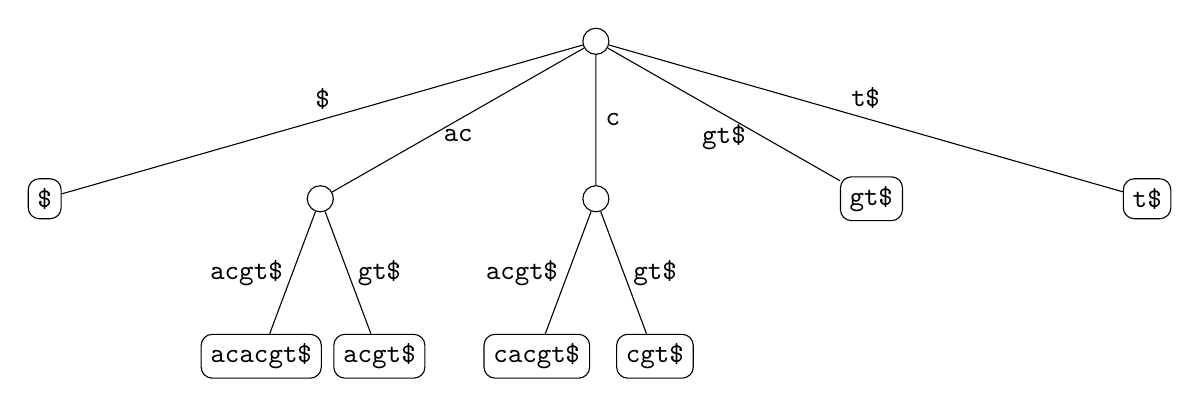
\begin{tikzpicture}
    [
        level 1/.style = {sibling distance = 3.5cm, level distance = 2cm},
        level 2/.style = {sibling distance = 1.5cm, level distance = 2cm}
    ]

        \node[draw, circle] {}
        child {
            node[draw, rounded corners] {\texttt{\$}}
            edge from parent node [above] {\texttt{\$}}
        }
        child {
            node[draw, circle] {}
            child {
                node[draw, rounded corners] {\texttt{acacgt\$}}
                edge from parent node [left] {\texttt{acgt\$}}
            }
            child {
                node[draw, rounded corners] {\texttt{acgt\$}}
                edge from parent node [right] {\texttt{gt\$}}
            }
            edge from parent node [below] {\texttt{ac}}
        }
        child {
            node[draw, circle] {}
            child {
                node[draw, rounded corners] {\texttt{cacgt\$}}
                edge from parent node [left] {\texttt{acgt\$}}
            }
            child {
                node[draw, rounded corners] {\texttt{cgt\$}}
                edge from parent node [right] {\texttt{gt\$}}
            }
            edge from parent node [right] {\texttt{c}}
        }
        child {
            node[draw, rounded corners] {\texttt{gt\$}}
            edge from parent node [below] {\texttt{gt\$}}
        }
        child {
            node[draw, rounded corners] {\texttt{t\$}}
            edge from parent node [above] {\texttt{t\$}}
        }
        ;
    \end{tikzpicture}
    \caption{suffixboom voor de string \texttt{acacgt\$}.}\label{fig:suffix_tree_example}

\end{figure}

Natuurlijk is dit niet efficiënt om effectief op deze manier op te slaan.
Als de tekst lengte $n$ heeft, heeft de suffixboom voor de tekst ten hoogste $2n - 1$ toppen en $2n - 2$ bogen.
Het aantal toppen en bogen is dus $\Theta(n)$.
Jammer genoeg vraagt alleen het opslaan van alle prefixen in de bladeren $\Theta(n^2)$ geheugen~\cite{AD3_ukkonen}.
In de plaats kunnen we pointers bijhouden naar het begin en einde van een substring in de originele string.
Dit zorgt er voor dat we geen kopie meer moeten opslaan van de originele string in elk blad.
Sterker nog, we moeten dit zelfs niet in elk blad bijhouden.
We kunnen simpelweg bij elke boog tussen de toppen de labels bijhouden.
Het label van het blad kunnen we daarna reconstrueren door de labels van de bogen op weg naar dit blad te achter elkaar te plaatsen.
Door dit te doen is de nodige opslag per top een constante, en is het geheugengebruik lineair.
Figuur~\ref{fig:suffix_tree_example_indices} toont hoe dit er in de praktijk uit ziet.
Merk op dat de eindindex exclusief is.
Een boog met waarde \texttt{1,3}, stelt dus de substring \texttt{ca} voor uit het voorbeeld.

\begin{figure}[H]
    \center
    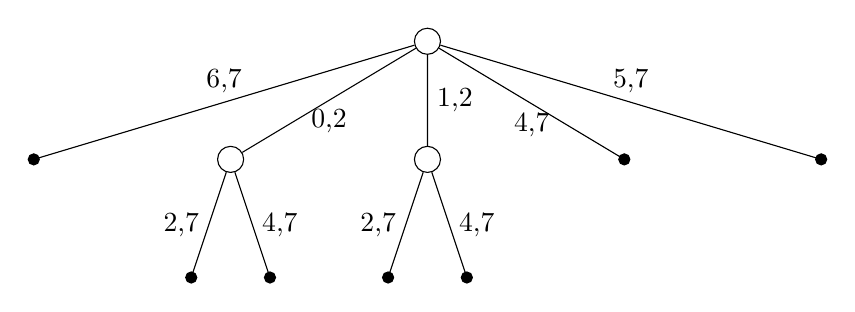
\begin{tikzpicture}
    [
        level 1/.style = {sibling distance = 2.5cm},
        level 2/.style = {sibling distance = 1cm}
    ]

        \node[draw, circle] {}
        child {
            [fill] circle (2pt)
            edge from parent node [above] {6,7}
        }
        child {
            node[draw, circle] {}
            child {
                [fill] circle (2pt)
                edge from parent node [left] {2,7}
            }
            child {
                [fill] circle (2pt)
                edge from parent node [right] {4,7}
            }
            edge from parent node [below] {0,2}
        }
        child {
            node[draw, circle] {}
            child {
                [fill] circle (2pt)
                edge from parent node [left] {2,7}
            }
            child {
                [fill] circle (2pt)
                edge from parent node [right] {4,7}
            }
            edge from parent node [right] {1,2}
        }
        child {
            [fill] circle (2pt)
            edge from parent node [below] {4,7}
        }
        child {
            [fill] circle (2pt)
            edge from parent node [above] {5,7}
        }
        ;
    \end{tikzpicture}
    \caption{suffixboom voor de string \texttt{acacgt\$} gebruik makende van indices.}\label{fig:suffix_tree_example_indices}

\end{figure}


\section{Het Algoritme van Ukkonen}\label{sec:Ukkonen}
Het algoritme van Ukkonen om suffixbomen op te bouwen~\cite{Ukkonen1995} is niet eenvoudig.
De pseudocode en de theoretische beschrijving in de originele paper zijn beide vrij complex.
Het algoritme komt echter uitgebreid aan bod in een heleboel andere publicaties en boeken~\cite{Gusfield1997, AD3_ukkonen, CCB_course, Ukkonen_CCB}.
Deze waren een erg grote hulp in het maken van een eigen eigen implementatie.

\subsection{Kotlin}\label{subsec:kotlin}
Ik ben begonnen met een implementatie van Ukkonen's algoritme in Kotlin zodat ik me niet op taal-specifieke problemen zou moeten focussen (vooral restricties rond \textit{borrowing} in Rust).
Hier was gelukkig de referentiecode van prof. Jan Fostier~\cite{Ukkonen_CCB} een grote hulp omdat dit het mogelijk maakte om tijdens het debuggen te zien wat de toestand van het programma is na $x$ stappen.
\\ \\
Één van de verschillen tussen mijn Kotlin implementatie en de referentie-implementatie is de manier waarop de kinderen voorgesteld worden.
In mijn implementatie is dit aan de hand van een HashMap in plaats van een array van pointers, simpelweg uit gemak zodat ik rechtstreeks een karakter als sleutel kon gebruiken, en die niet moest omzetten naar een index.
Om dit prototype te maken heb ik gekozen voor Kotlin boven Python aangezien Kotlin performanter is en ook een aangename ontwikkelingservaring biedt.
Hierdoor is het mogelijk om toch de test datasets op te bouwen in een redelijke tijd.
\\ \\
Uiteindelijk bleek de grootste struikelblok in het implementeren van Ukkonen enkele off-by-1 fouten.
Aangezien je tijdens het algoritme eigenlijk werkt met substrings, maar deze opgeslagen worden aan de hand van hun begin- en eindindex wordt het debuggen veel omslachtiger.
Tot slot had ik op het einde ook enkele bugs die niet voorkwamen in kleinere voorbeelden die met de hand uit te werken waren, wat daardoor relatief wat tijd vroeg om op te lossen.

\subsection{Rust}\label{subsec:rust}

\subsubsection{Boomstructuren}
\begin{quote}
    \textit{Rust is known to be notorious difficult when it comes to certain data structures like linked lists, trees, etc. \cite{rust_difficulty_quote}}
\end{quote}
Deze quote komt rechtstreeks uit een Medium artikel en toont direct aan dat het maken van een suffixboom in Rust niet-triviaal ging zijn.
De oorzaak hiervoor ligt bij het \textit{ownership} systeem van Rust.
Dit systeem zorgt er voor dat slechts één variabele eigenaar kan zijn van een stukje data.
In dit geval kan dus slechts één top een andere top opslaan, of er een \textit{mutable reference} naar hebben.
Meer praktisch wil dit dus zeggen dat slechts één top een \textit{pointer} kan hebben naar een andere top, met de toelating om die top aan te passen (wat nodig is tijdens het opbouwen van de boom. Er worden namelijk nog kindere toegevoegd en toppen gesplitst).
Dit is een groot probleem aangezien ouders pointers naar kinderen moeten hebben, de kinderen een pointer naar hun ouder, en er dan ook nog eens pointers zijn voor de suffix links.
\\ \\
Als oplossing hiervoor introduceert Rust het \texttt{Rc<T>} datatype.
Hierbij gaat Rust afstappen van zijn standaard \textit{ownership} systeem en gebruik maken van Reference Counting.
Pas wanneer alle referenties weg zijn zal het geheugen automatisch vrijgegeven worden.
De beperking hierbij is echter dat deze referenties \textit{immutable} zijn, dit volstaat niet tijdens het opbouwen van de boom.
\\ \\
Als oplossing hiervoor heeft Rust dan weer het \textit{interior mutability} patroon~\cite{interior_mutability} aan de hand van het datatype \texttt{Refcell}.
Dit laat toe om data toch aan te passen, ook al is de referentie \textit{immutable}.
Aangezien dit de standaard Rust regels doorbreekt, is dit \texttt{unsafe}\footnote{Dit is code waarvan de compiler niet kan nagaan als die aan alle voorwaarden voldoet die nodig zijn om \textit{memory safety} te kunnen garanderen. Dit sleutelwoord bestaat zodat de programmeur meer vrijheid zou kunnen krijgen om bepaalde patronen toch toe te kunnen passen. De verantwoordelijkheid om correct het geheugen te gebruiken wordt hier bij de programmeur gelegd. Een andere reden om \texttt{unsafe} te gebruiken is om bepaalde interacties met hardware uit te voeren. Deze zijn inherent onveilig en zouden anders onmogelijk zijn.} en kan Rust \textit{at compile-time} geen \textit{memory safety} meer garanderen.
\texttt{Refcell} zal gelukkig wel de nodige code invoegen zodat runtime memory safety wel gegarandeerd kan worden.
Mogelijke foutieve geheugen operaties zullen dus tijdens het uitvoeren van het programma gedetecteerd worden, \textbf{ten koste van performantie}.
\\ \\
Maar zelfs nu blijft er nog altijd een probleem.
Geheugen dat beheerd wordt aan de hand van \textit{reference counting} zal enkel vrijgegeven kunnen worden indien de \textit{reference counter} op 0 staat.
Er zijn echter scenario's waar dit nooit zal gebeuren.
Namelijk bij cyclische verwijzingen, een patroon dat jammer genoeg erg vaak voor komt (in ons geval bv. een ouder die een pointer heeft naar een kind, en een kind een pointer naar de ouder).
Als oplossing hiervoor introduceert Rust dan weer het \texttt{Weak<T>} datatype.
\\ \\
Dit is duidelijk erg ingewikkeld, en introduceert ook nog eens \textit{performance overhead} die niet nodig lijkt.
Een optie zou natuurlijk zijn door expliciet het \texttt{unsafe} keyword te gebruiken wat toe laat de ownership regels van Rust volledig uit te schakelen (zowel tijdens het compileren als tijdens het uitvoeren).
Het nadeel hiervan is natuurlijk dat we dan de garanties van memory safety kwijt zijn, wat net één van de hoofdredenen is om Rust te gebruiken.
Dit was dus geen mogelijke optie.
Gelukkig is er een alternatieve manier waar ik op gestoten ben, een \textit{arena-based} implementatie~\cite{rust_arena_trees}.
Het idee hierbij is dat er één arena gemaakt wordt waarbij ownership erg simpel is.
In mijn implementatie is dit bijvoorbeeld een \texttt{Vector}.
Alle toppen worden hierbij in deze ene vector opgeslagen.
In plaats van pointers naar elkaar houden bij te houden zullen de toppen indexen bijhouden.
Deze index stelt de index in de arena van de top voor waarnaar anders een pointer wordt bijgehouden.
\\ \\
Na het maken van deze ontwerpaanpassingen bleef slechts één moeilijkheid over.
Uitzoeken hoe de cursor (die bijhoudt waar we zijn in de boom tijdens het bouwen), de input string en de boom zelf zich van elkaar moeten verhouden in het ownership systeem.
Uiteindelijk viel dit vrij makkelijk uit te zoeken.
Het omzetten van de resterende Kotlin code naar Rust was erg simpel en bijna een één op één vertaling.
Het enige verschil is dat ik in de Rust implementatie gebruik heb gemaakt van een array om de kinderen bij te houden in plaats van een HashMap.

\subsubsection{Geheugen efficiëntie}
\begin{quote}
    \textit{And then I went and invented a null pointer.
    And if you use a null pointer you either have to check every reference or you risk disaster. \cite{null_mistake}}
\end{quote}
\textit{Null pointers} worden ook wel \textit{the billion-dollar mistake} genoemd vanwege het grote aantal bugs dat ze veroorzaken.
Daarom voorziet Rust een andere manier om de waarde \textit{null} voor te stellen.
Dit wordt gedaan aan de hand van de \texttt{Option<T>} enum.

\begin{minted}{Rust}
enum Option<T> {
    None,
    Some(T),
}
\end{minted}

Deze enum heeft 2 mogelijke waarden: \texttt{None} of \texttt{Some(T)}.
\texttt{None} is het equivalent van \textit{null}, terwijl \texttt{Some(T)} wil zeggen dat de waarde verschillend is van null, meer specifiek is de waarde \texttt{T}.
Aangezien het grootste deel van wat bijgehouden wordt per top eigenlijk pointers zijn maakte ik veelvoudig gebruik van deze Option-enum.
Alle pointers in een top kunnen namelijk \textit{null} zijn.
De \textit{parent pointer} moet nullable zijn aangezien de root geen ouder heeft, de \textit{child pointers} moeten allemaal nullable zijn omdat bladeren geen kinderen hebben (en in de interne toppen zijn niet alle kinderen altijd nodig) en de suffix links moeten nullable zijn aangezien niet elke top een suffix link heeft naar een andere top.
\\ \\
Dit werkte perfect en kon mooi afgehandeld worden op de idiomatische manier die overeenkomt met goede Rust code.
Na de eerste benchmarks bleek het geheugengebruik echter problematisch.
Bijna exact 2x zo hoog als de equivalente C++ implementatie.
Om zo'n drastisch verschil in geheugenverbruik te kunnen verklaren moest er wel iets fundamenteel verschillen aan de manier dat toppen hun data bijhouden.
Al snel bleek dat het gebruik van \texttt{Option<usize>} als datatype in plaats van \texttt{usize} 8 bytes aan overhead per index had.
Dit is inderdaad exact het dubbele geheugenverbruik op een 64-bit machine aangezien een \texttt{usize} 8 bytes groot is.
Dit valt makkelijk te controleren aan de hand van de \texttt{std::mem::size\_of} functie, deel van de Rust standaard bibliotheek.
Onderstaand voorbeeld toont dat dit inderdaad het geval is.
\begin{minted}{Rust}
assert_eq!(mem::size_of::<Option<usize>>(), 16);
assert_eq!(mem::size_of::<usize>(), 8);
\end{minted}

Als oplossing heb ik uiteindelijk mijn eigen \textit{null} waarde gedefinieerd gebruik makende van een \textit{trait}\footnote{Een trait in Rust definieert een functionaliteit dat een bepaald type heeft, en kan delen met andere types}.
Deze oplossing verslaat volledig het doel van de \texttt{Option<T>} enum, maar is jammergenoeg nodig omdat het gewoonweg niet acceptabel is het geheugenverbruik te verdubbelen hiervoor.
Bovendien blijft memory safety gegarandeerd aangezien het foutief indexeren van de NULL-value (\texttt{usize::MAX} in dit geval) een index-out-of-bounds error creëert.
Wat tijdens runtime gedetecteerd wordt en dus geen verdere problemen geeft (afgezien van een mogelijke crash van het programma).

\begin{minted}{Rust}
/// Custom trait implemented by types that have a value that represents NULL
pub trait Nullable<T> {
    const NULL: T;

    fn is_null(&self) -> bool;
}

/// Type that represents the index of a node in the arena part of the tree
pub type NodeIndex = usize;

impl Nullable<NodeIndex> for NodeIndex {
    /// Use usize::MAX as NULL value since this will in practice never be reached.
    /// It is not possible to create 2^64-1 nodes (on a 64-bit machine).
    /// This would simply never fit in memory
    const NULL: NodeIndex = usize::MAX;

    fn is_null(&self) -> bool {
        *self == Self::NULL
    }
}
\end{minted}

\subsection{Performantie}\label{subsec:performantie}
Natuurlijk is het belangrijk dat de implementatie performant (en correct) is.
Aangezien we ook over een bestaande C++ implementatie van Ukkonen's algoritme beschikken, was dit een perfecte maatstaf.
Uiteindelijk heb ik één aanpassingen moeten maken in deze C++ code om een eerlijke vergelijking uit te voeren.
Oorspronkelijk werd er in elke top plaats gehouden voor 256 mogelijke kinderen.
Dit was veel te hoog voor onze use case.
Er zijn nl. slechts 20 aminozuren en enkele \textit{wildcard characters}.
Dit verklaart onmiddellijk waarom het geheugengebruik ongeveer een factor 10 hoger was dan nodig.
Uiteindelijk ben ik gegaan voor een implementatie (zowel in Rust als C++) waarin plaats gehouden wordt voor 28 kinderen.
Dit zijn de 26 letters van het alfabet + \texttt{`\#`} + \texttt{`\$`}.
\texttt{`\#`} en \texttt{`\$`} worden gebruikt als resp. scheidingsteken en eindteken.
Dit is ook wat al gebeurde in de bestaande C++ implementatie.
\\ \\
Een andere aanpak zou kunnen zijn om HashMaps te gebruiken.
Het totale geheugenverbruik zal hierdoor afnemen naar ongeveer 60\% van het huidige verbruik, maar ten koste van performantie tijdens het zoeken (wat net erg belangrijk is).
Hoe dan ook blijft het geheugen verbruik extreem groot, welke implementatie ook gekozen wordt.
\\ \\
Het vergelijken van de implementaties heb ik opgesplitst in 2 stukken:
\begin{enumerate}
    \item het opbouwen van de indexstructuur.
    \item Zoeken in de indexstructuur
\end{enumerate}

\subsubsection{Opbouwen}
Om een representatief resultaat te krijgen is het opbouwen van de boom 10x uitgevoerd en zijn de gemiddelden van de resultaten genomen.
Om de uitvoeringstijd en het geheugenverbruik te meten heb ik gebruik gemaakt van het \texttt{time} commando.
De resultaten hiervan zijn terug te vinden in figuur~\ref{fig:tree_building}.
\begin{figure}[H]
    \centering
    \subfloat[Tijd nodig om de suffixboom op te bouwen]{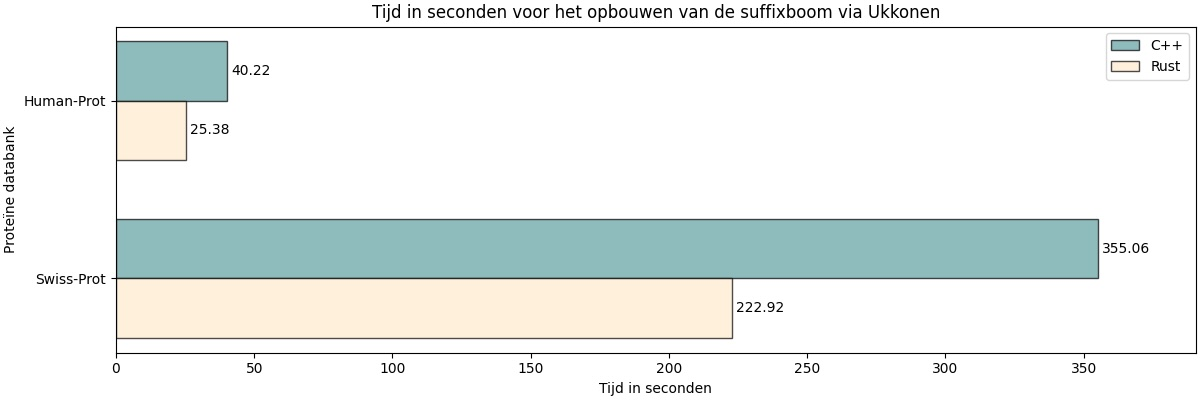
\includegraphics[width=\linewidth]{building_tree_time}}\\[4ex] % [4ex] om wat extra vertical spacing in te voegen

    \subfloat[Maximaal gebruikt geheugen tijdens het opbouwen van de suffixboom]{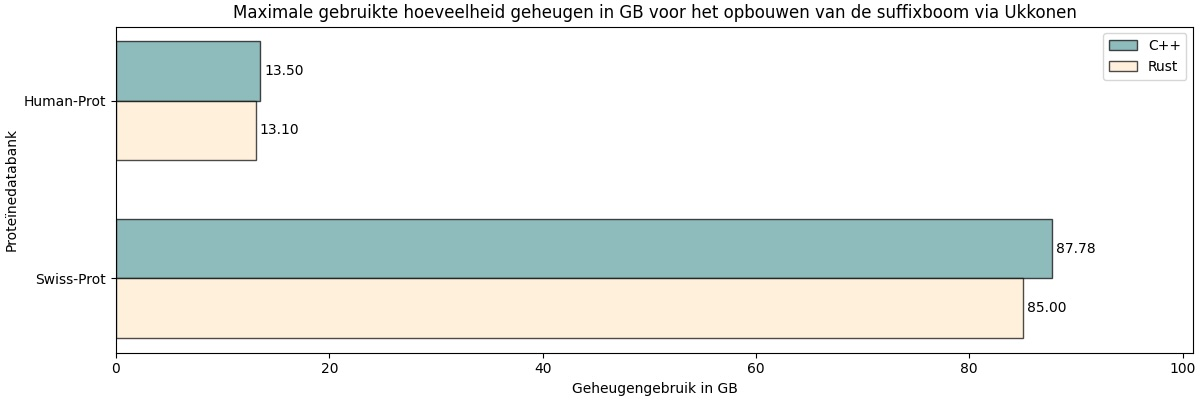
\includegraphics[width=\linewidth]{building_tree_memory}}
    \caption{Vergelijking van C++ en Rust voor het opbouwen van de suffixboom. De tijd en het geheugengebruik is gemeten gebruik makende van het \texttt{time} commando met als invoerbestand de Swiss-Prot of Human-Prot eiwitdatabank.}\label{fig:tree_building}
\end{figure}

Uit deze grafieken vallen 2 duidelijke conclusies te trekken.
\begin{enumerate}
    \item De implementatie in Rust is $\pm$ 33\% sneller
    \item Het geheugenverbruik is erg vergelijkbaar.
    Dit valt te verwachten aangezien beide implementaties 8 bytes nodig hebben per \textit{pointer} en evenveel plaats voorzien voor de kinderen.
    Het kleine verschil valt te verklaren vanwege 1 veld dat ik niet bij houdt tijdens het opbouwen, dat wel gebruikt wordt in de C++ implementatie.
    Dit is de diepte van de top in de boom.
    Op de enkele plaatsen waar dit nodig is kan ik gebruik maken van andere variabelen om tot een equivalent resultaat te komen.
\end{enumerate}

\subsubsection{Zoeken}
Bij het zoeken zijn er 2 belangrijke manieren om te vergelijken.
\begin{enumerate}
    \item Zoek totdat we weten als er een match bestaat voor de peptide of niet, en stop dan.
    \item Zoek totdat er een match is, en doorzoek daarna de volledige subboom om alle informatie van de kinderen op te halen.

\end{enumerate}

\paragraph{Zoek een match}
De reden voor deze manier van zoeken is dat het mogelijk is om info te propageren van de bladeren tot bovenin de boom.
In ons geval is dit bijvoorbeeld de LCA\footnote{Lowest Common Ancestor} van de taxon IDs op voorhand te berekenen.
Het zoeken van de LCA die overeenkomt met alle proteïnen waar de gevonden peptide mee matcht kan dus al stoppen vanaf er een match is.
\\ \\
Grafiek~\ref{fig:performance_match_tree} toont de nodige tijd om alle peptiden van de gebruikte zoekbestanden éénmalig te zoeken totdat er een (mis)match was voor de peptide.
De grafiek bevat de gemiddelde resultaten van 5000 uitvoeringen, maar zelfs dan bleven de resultaten wat schommelen.
Doordat de te meten tijd zo klein is, kan de kleinste invloed van omgevingsfactoren al voor een zichtbaar verschil zorgen.
Dit kan bv. een achtergrondproces zijn, maar ook invloed van een andere VM die op de fysieke machine bezig is.
Dit was ook merkbaar tijdens het testen waar dat de verschillen tussen 2 opeenvolgende uitvoeringen vaak groter waren dan het verschil tussen de C++ en Rust implementatie.
Toch kunnen we besluiten dat de C++ implementatie een beetje performanter is aangezien dit in elk zoekbestand (nipt) sneller is (soms zelfs minder dan een milliseconde).

\begin{figure}[H]
    \centering
    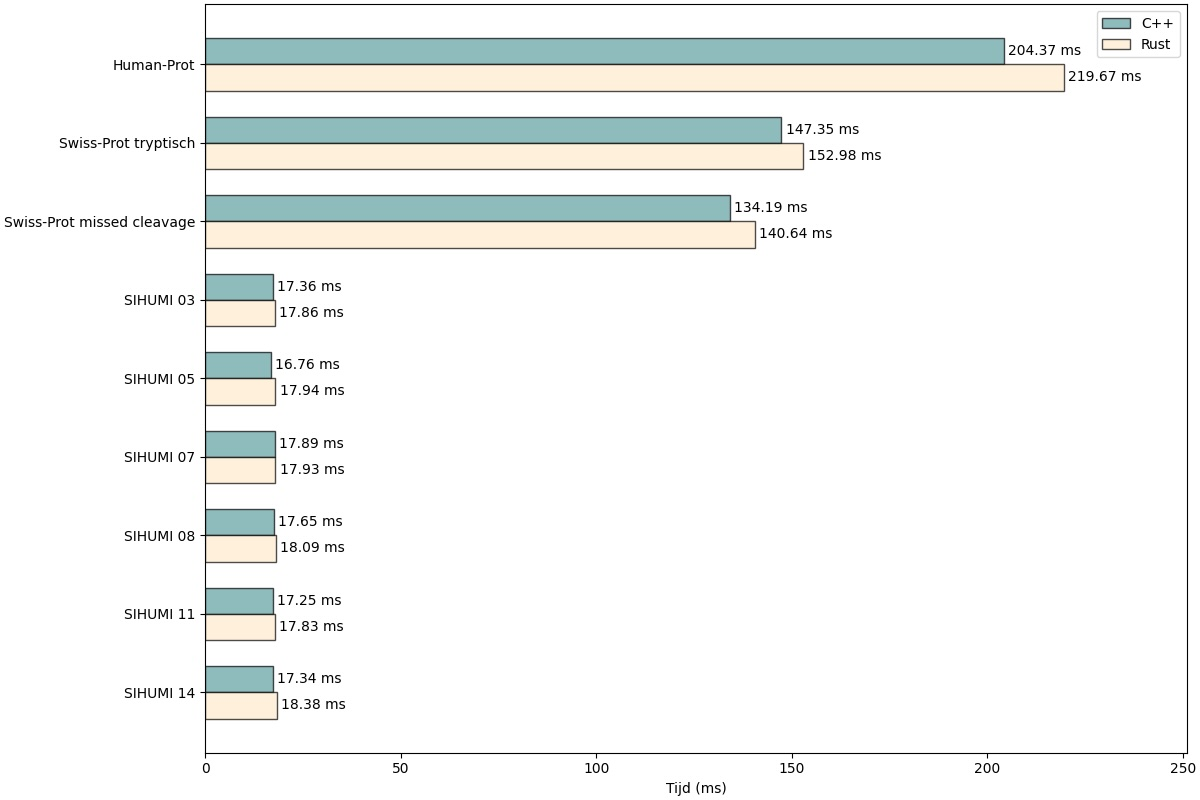
\includegraphics[width=\linewidth]{search_match_performance_tree}
    \caption{Uitvoeringstijd in milliseconden voor het zoeken tot een match voor alle zoekbestanden. Deze resultaten zijn het gemiddelde van 5000 uitvoeringen. Één iteratie wordt gezien als één maal elke peptide die deel is van het zoekbestand te zoeken in de suffixboom, en te stoppen wanneer er een (mis)match gevonden is. Het meten van de tijd is gebeurd in de code zelf.}
    \label{fig:performance_match_tree}
\end{figure}

Het verschil met de huidige implementatie van Unipept is gigantisch.
Daar duurt het op dit moment 2 minuten en 12 seconden om alle peptiden van het Swiss-Prot zoekbestand zonder \textit{missed cleavages} te zoeken,
en maar liefst 30 minuten 37 seconden voor het zoekbestand met \textit{missed cleavages}!
Dit is maar liefst $\frac{132 000}{152.98} = 857$ en $\frac{1 837 000}{140.64} = 13 000$ keer trager!
Als keerzijde van de medaille gebruikt Unipept op dit moment hiervoor slechts 6.7 GiB geheugen, en dit kan zelfs nog naar beneden.
Dit is ongeveer 13 keer lager!

\paragraph{Zoek match en haal informatie over kinderen op}
De reden dat dit belangrijk is, is dat alle bladeren in deze subboom de proteïnen voorstellen waar dat de gevonden peptide een deel van is.
De relevante informatie over de huidige peptide is daarom de informatie die verbonden is met deze proteïnen.

Figuur~\ref{fig:performance_all-occurrences_tree} bevat een overzicht van de nodige zoektijd voor beide implementaties op alle zoekbestanden.
We zien duidelijk dat er hier een gigantisch verschil is tussen de C++ en Rust implementatie.
Vermoedelijk komt dit door de andere \textit{memory layout} die ontstaat doordat de Rust implementatie 1 grote Vector gebruikt, terwijl de C++ implementatie losse toppen gebruikt die verspreid liggen in het geheugen.

\begin{figure}[H]
    \centering
    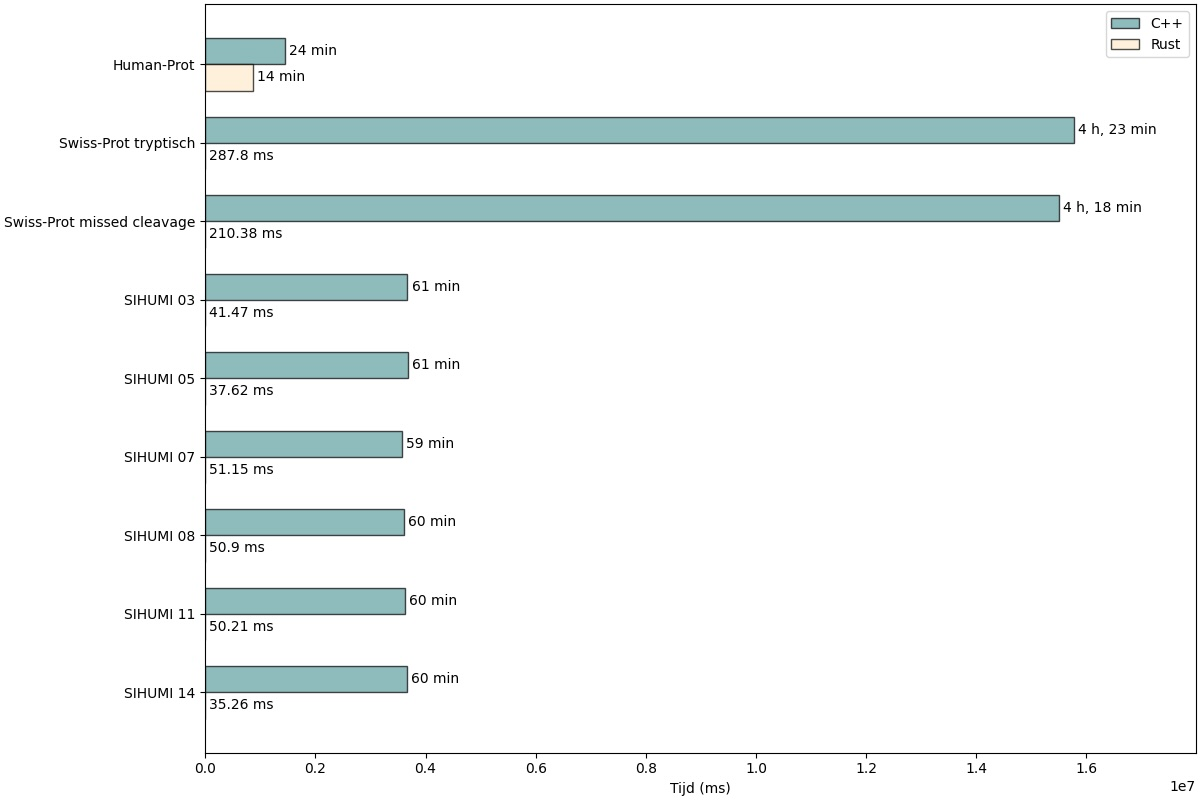
\includegraphics[width=\linewidth]{search_all-occurrences_performance_tree}
    \caption{Uitvoeringstijd inclusief het doorzoeken van de volledige subboom na match voor alle zoekbestanden. Deze resultaten zijn het gemiddelde van 10 uitvoeringen. 1 iteratie wordt gezien als 1x elke peptide die deel is van het zoekbestand te zoeken in de suffixboom, en bij een match de volledige resterende subboom te doorzoeken. Dit toont de tijd die nodig is om informatie uit de bladeren op te halen voor alle proteïnen waar een peptide substring van is. Het meten van de tijd is gebeurd in de code zelf.}
    \label{fig:performance_all-occurrences_tree}
\end{figure}


\section{Taxon ID aggregatie}\label{sec:taxon-id-aggregatie}
Één van de belangrijkste analyses die Unipept aanbiedt, is de taxonomische analyse waarin uitgezocht wordt met welke organismen de peptiden uit een staal overeenkomen.
Aangezien peptiden kunnen matchen met proteïnen die uit verschillende organismen komen moet er een manier gekozen worden om deze informatie te aggregeren, of te beslissen van welk organisme dit komt met de grootste kans.
Aangezien er geen manier is om met zekerheid te zeggen uit welke proteïne de peptide komt (als er meerdere opties zijn) gaat Unipept de info conservatief veralgemenen.
Anders gezegd: Unipept zal enkel info geven die geldt voor alle gematchte proteïnen.
Één van deze stukjes informatie is het Taxon ID\@.
In plaats van een lijst van alle mogelijke IDs te geven (wat een extreem grote lijst kan zijn), en wat zou vereisen de volledige subboom na het vinden van een match af te lopen, gaan we deze taxon IDs gaan aggregeren aan de hand van een strategie gebruik makende van de NCBI taxonomy database~\cite{NCBI_original_article, NCBI_update}.
Met andere woorden, we gaan dus op zoek naar de kleinste gemeenschappelijke voorouder van alle taxon IDs die in de bladeren van de subboom zitten van een bepaalde top.
Hiervoor bestaan verschillende strategieën die al uitgewerkt zijn in UMGAP, en die hier herbruikbaar waren.
\\ \\
Origineel was het plan om LCA* te gebruiken als aggregatie strategie.
Dit is een heuristiek om de LCA (lowest common ancestor) te berekenen.
Hierbij zoeken we de meest specifieke taxon in de boom die ofwel een ouder of kind is van elke taxon in de boom.
Anders gezegd is dit de LCA van een lijst taxa, nadat we alle taxa verwijderd hebben die ouder zijn van minstens één taxon in die lijst~\cite{UMGAP_paper}.
Het voordeel hiervan is dat we iets langer exactere info kunnen behouden.
Want bij LCA zelf zal het resultaat altijd 1 zijn vanaf één top in de subtree dit als LCA heeft (1 is namelijk ouder van alle andere taxons!).
\\ \\
Het idee was dat we niet elke keer naar de bladeren moeten gaan om het taxon ID te berekenen van één top, maar dat dit ging kunnen op basis van de taxon IDs van de directe kinderen van de top.
Op deze manier gingen we met één bottom-up sweep van de boom alle taxon IDs kunnen berekenen.
Dit bleek echter niet mogelijk omdat gebruik maken van de directe kinderen een ander resultaat geeft dan gebruik maken van de bladeren van de subboom.
Figuur~\ref{fig:lca*_diff} toont een minimaal voorbeeld uitgewerkt voor beide strategieën.
De licht grijze toppen zijn ingevuld zijn aan de hand van aggregatie, terwijl de zwarte toppen gegeven zijn.

\begin{figure}[H]
    \centering
    \subfloat[LCA* op basis van de bladeren]{
        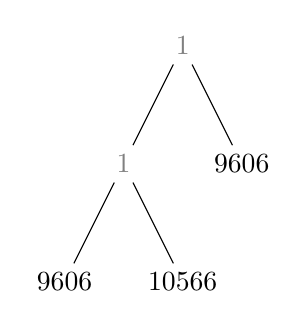
\begin{tikzpicture}
            \node [gray] {1}
            child {node [gray] {1}
            child {node {9606}}
            child {node {10566}}}
            child {node {9606}
            };
        \end{tikzpicture}
    }\hspace{0.25\textwidth}%
    \subfloat[LCA* op basis van de kinderen]{
        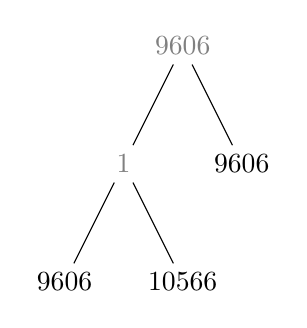
\begin{tikzpicture}
            \node [gray] {9606}
            child {node [gray] {1}
            child {node {9606}}
            child {node {10566}}}
            child {node {9606}
            };
        \end{tikzpicture}
    }
    \caption{Minimaal voorbeeld van de 2 aggregatie manieren gebruik makende van LCA*. De grijze toppen zijn berekend aan de hand van een LCA*, terwijl de zwarte toppen gegeven zijn.}\label{fig:lca*_diff}
\end{figure}

Onderstaande uitleg behandelt de werkwijze voor bovenstaande figuren.
\begin{itemize}
    \item Het toepassen van LCA* voor het berekenen van de top op basis van de bladeren van de boom (\{9606, 10566, 9606\}) heeft als resultaat 1 voor de root van de boom.
    9606 en 10566 zijn geen ouder of kind van elkaar, dus zal LCA* hetzelfde doen als LCA\@.
    De kleinste gemeenschappelijke ouder van deze 2 taxons is 1.
    \item Het toepassen van LCA* op basis van de directe kinderen geeft als resultaat 9606.
    Dit val simpel te verklaren aangezien de LCA* van de linker subboom 1 is.
    Als we daarna dan de LCA* van \{1, 9606\} nemen wordt 1 verwijderd aangezien dit een ouder is van 9606.
    De LCA van 9606 is natuurlijk gewoon zichzelf!
\end{itemize}

Het berekenen van de LCA* op de eerste manier is echter niet schaalbaar voor de volledige suffixboom.
Om een idee van grootorde te geven: de suffixboom voor de Swiss-Prot dataset bevat 328 922 516 toppen in het totaal, waarvan 206 523 693 bladeren.
\\ \\
Daarom hebben we uiteindelijk toch voor de standaard LCA aggregatie manier gekozen.
Deze laat wel toe de toppen op deze efficiëntere manier te aggregeren.
UMGAP biedt 2 manieren aan om LCA te doen.
Gebruik makende van RMQ (Range Minimum Queries) en een boom-gebaseerde structuur.
Zelf maak ik gebruik van de RMQ implementatie aangezien deze significant sneller was (8 min 58 sec vs 20 min en 25 sec voor de Swiss-Prot databank).
Tot slot heb ik ook eens vergeleken hoe groot de behaalde tijdswinst is bij het gebruik kunnen maken van de directe aggregatie op de kinderen, vergeleken met aggregatie op basis van de bladeren.
Bij het aggregeren op basis van de bladeren met de RMQ implementatie was de uitvoeringstijd maar liefst 12 uur, 19 minuten en 16 seconden!
Dit is dus een extreem groot verschil.

\section{Conclusie suffixbomen}\label{sec:conclusie-suffix-bomen}
Het is duidelijk dat suffixbomen erg performant zijn voor dit scenario.
Het opbouwen gebeurt snel en het zoeken voor een match gaat vliegensvlug.
\\ \\
Door de eigen implementatie in Rust kunnen we ook wat tijd besparen ten opzichte van een equivalente C++ implementatie.
Een deel van de winst zit tijdens het opbouwen van de boom, maar vooral tijdens het zoeken wanneer informatie uit de bladeren gehaald moet worden.
Vermoedelijk ligt de andere geheugenstructuur hiervoor aan de basis.
\\ \\
Ondanks de veelbelovende resultaten op vlak van snelheid is er een keerzijde aan de medaille.
Het geheugengebruik is zo groot dat we op zoek moeten naar een andere datastructuur.
Voor de Swiss-Prot databank gaat het geheugenverbruik al boven 80 GB, terwijl ons einddoel is om dit te gebruiken op de TrEMBL dataset.
Dit wilt zeggen dat als we alles \textit{slechts} $\pm$ 500 maal kunnen opschalen het doel bereikt is.
Dit zou echter vereisen dat we een server hebben met ongeveer 50 TB aan RAM geheugen.
Dit is niet mogelijk, we moeten daarom op zoek naar een andere datastructuur die minder geheugen vereist.
